% flashcards-title: Two positions on a signed number line
% flashcards-desc: A line from negative four to positive four marks P at negative three and Q at positive two, with zero centered.
\documentclass[dvisvgm,tikz,border=8pt]{standalone}
\usetikzlibrary{arrows.meta,patterns}

\definecolor{qraNavy}{HTML}{17324D}
\definecolor{qraBlue}{HTML}{2B6CB0}
\definecolor{qraGold}{HTML}{B7791F}
\definecolor{qraPale}{HTML}{EAF2F8}
\definecolor{qraGray}{HTML}{5C6773}

\tikzset{
  qra axis/.style={draw=qraNavy, line width=1.2pt},
  qra tick/.style={draw=qraNavy, line width=1pt},
  qra guide/.style={draw=qraGray, densely dashed, line width=0.8pt},
  qra counter/.style={circle, draw=qraNavy, fill=qraPale, line width=0.9pt, minimum size=7mm, inner sep=0pt},
  qra label/.style={font=\sffamily\bfseries, text=qraNavy},
  qra small label/.style={font=\sffamily, text=qraNavy},
}

\begin{document}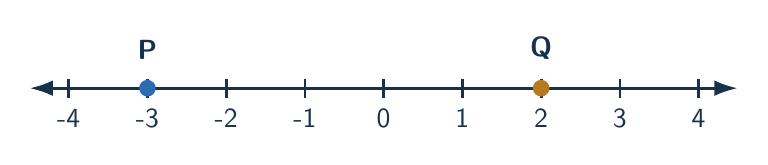
\begin{tikzpicture}[x=1cm,y=1cm]
\draw[qra axis,{Latex[length=3mm,width=2mm]}-{Latex[length=3mm,width=2mm]}](-4.5,0)--(4.5,0);
\foreach \x in {-4,...,4}{\draw[qra tick](\x,-.12)--(\x,.12);\node[qra small label,below=4pt] at(\x,0){\x};}
\fill[qraBlue](-3,0)circle(3pt);\node[qra label,above=7pt]at(-3,0){P};
\fill[qraGold](2,0)circle(3pt);\node[qra label,above=7pt]at(2,0){Q};
\end{tikzpicture}\end{document}
